\documentclass[a4paper,11pt]{article}
\usepackage[utf8]{inputenc}
\usepackage[T1]{fontenc}
\usepackage{amsmath}
\usepackage{mathtools}
\usepackage{amsfonts}
\usepackage{amssymb}
\usepackage{graphicx}
\usepackage{multicol}
\usepackage{array}
\usepackage{float}
\usepackage{epstopdf}
\usepackage{caption}
\usepackage{subcaption}
\usepackage{gensymb}
\usepackage[bottom]{footmisc}
\usepackage{appendix}
\usepackage{pdfpages}
\usepackage{todonotes}
\usepackage{mathpazo}
\usepackage{titleps}
\usepackage{color}
\usepackage{xcolor}
\usepackage{colortbl}
\usepackage{siunitx}
\usepackage{pdflscape}
\usepackage{cancel}

\usepackage[skins]{tcolorbox}
\usepackage{sectsty}
\usepackage[arrowmos]{circuitikz}
\usepackage{pgfplots}
\usepackage{blindtext}
\usepackage[inner=2cm,outer=2cm,top=2.5cm,bottom=2.5cm]{geometry}
\usepackage{todonotes}
\usepackage{hyperref}
\usepackage{url}
\usepackage{adjustbox}
\usepackage{tabularx}
\usepackage{booktabs}
\usepackage{fancybox}
\usepackage[tikz]{bclogo}



%For code insertion
%listing
\usepackage{listings}
\usepackage{xcolor}
\definecolor{codegreen}{rgb}{0,0.6,0}
\definecolor{codegray}{rgb}{0.5,0.5,0.5}
\definecolor{codepurple}{rgb}{0.58,0,0.82}
\definecolor{backcolour}{rgb}{0.98,0.98,0.98}
\lstdefinestyle{mystyle}{
    backgroundcolor=\color{backcolour},
    commentstyle=\color{codegreen},
    keywordstyle=\color{blue},
    numberstyle=\tiny\color{codegray},
    stringstyle=\color{codepurple},
    basicstyle=\ttfamily\footnotesize,
    breakatwhitespace=false,
    breaklines=true,
    captionpos=b,
    keepspaces=true,
    numbers=left,
    numbersep=5pt,
    showspaces=false,
    showstringspaces=false,
    showtabs=false,
    tabsize=2
}
\lstset{style=mystyle}



\graphicspath{{figures/}}
\sectionfont{\large}
\subsectionfont{\normalsize}



%%%%%%%%%%%%%%%%%%%
% HANDS-ON NUMBER
\newcommand\handsOnN{FPGA}
% WEEK NUMBER
\newcommand\weekN{8}
%%%%%%%%%%%%%%%%%%%

\newpagestyle{main}{
	\sethead[LELEC2102: Hands-on \handsOnN][][Week \weekN]{LELEC2102: Hands-on \handsOnN}{}{Week \weekN}
	\headrule
    \setfoot[][\thepage][]{}{\thepage}{}
}

\newcommand{\horrule}[1]{\rule{\linewidth}{#1}} % Create horizontal rule command with 1 argument of height
%\setlength {\marginparwidth }{2cm}
%%%%%%%%%%%%%%%%%%%%%%%%%%%%%%%%%%%%%%%%%%%%%%%%%%%%%%%%%%%%%%%%%%%%%%%%%%%%

\begin{document}
\renewcommand{\figurename}{Fig.}

\renewcommand{\thepage}{\arabic{page}}
\setcounter{page}{1}
\pagestyle{main}
\newpage \clearpage

\begin{center}
\begin{LARGE}
LELEC2103: Optimization
\end{LARGE}
\vspace{0.3cm}
%\textit{TA 1, TA 2}
\end{center}

\section*{Introduction}

In this hands-on, you will learn how to demodulate wireless transmissions using a software-defined radio (SDR).
In the final application, the S2LP radio of the MCU transmits to a gateway that embeds an FSK receiver.
This receiver runs in GNU Radio and uses the LimeSDR Mini, a SDR board, to recover the
baseband samples of the transmitted packet. The received samples are demodulated using the open source SDR \href{https://wiki.gnuradio.org/index.php/Main_Page}{GNU Radio software}.
To this end, the teaching team developed a full GNU Radio implementation\footnote{At the exception of the demodulation and CFO estimation functions that you wrote previously.}
of a FSK receiver compatible with the S2LP radio used in the project.
The main objective of this hands-on is to experimentally receive packets from the S2LP radio and to demodulate them in GNU Radio.

\section*{Objectives}

\begin{itemize}
    \item Discover the Nucleo MCU board and its programming tools ;
    \item Learn the basics of bare metal embedded programming, General-Purpose Inputs-Outputs (GPIOs), interrupts and timers ;
    \item Understand qualitatively and measure quantitatively how the embedded software program impacts the MCU power consumption ;
    \item Learn how to debug an embedded program by logging/tracing and using a physical debugger.
\end{itemize}

%\section*{Material}

\begin{comment}[couleur = gray!20, arrondi = 0.2, logo=\bcinfo]{}
\vspace{0.2cm}
\end{comment}
For this hands-on session, you will need:
\begin{itemize}
    \item The latest version of STM32 Cube IDE installed on your host system (for further information, see INSTALL.md on the GitHub of the course) ;
    \item The Nucleo MCU board with its sensing and power-management board ;
    \item A USB cable to connect your computer to the Nucleo.
\end{itemize}
%\vspace{0.01cm}

\section{Accelerating the detection of the preamble}
In the previous Hands-On, our demodulation chain required a component called the \textit{preamble detector} that actively seeks the preamble sequence located at the beginning of a packet by looking at the energy of each sample and accumulating it over time. When the accumulated value exceeded a threshold, the preamble was considered present and a given amount of samples were forwarded to the synchronization stage. This system allows to avoid unnecessary heavy computations as well as real-time operation. There are two drawbacks to this process. First, the threshold is not updated and increasing the gain of the RF front-end will increase the noise power, possibly going above the set threshold. Second, this preamble detection scheme requires a lot of computation, calculating and accumulating the energy of each sample. \\

As it operates continuously, it is best to move its functionality from software towards a specialized piece of hardware in order to improve its \textbf{energy efficiency and processing speed}. If we decide at one point to increase the packet rate of the overall transmission chain, this solution is more robust regarding packet misses. It is also further motivated by the fact that this block occurs at the very beginning of the processing chain, just after the low-pass filter. We will also change the behavior of the block by calculating the threshold based on the noise power and on a programmable margin coefficient. The accelerated block will therefore be called the packet presence detector (PPD). However, we only want to accelerate the energy detection step but still receive all samples in GNU Radio to be able to monitor the channel if needed. Therefore, the PPD will add a flag at the start of a packet when it has been detected. This flag corresponds to the value \texttt{0x7FF} which can not be practically reached by the LMS7002M chip.


\subsection{Design overview}
We implemented for you a packet presence detection module in SystemVerilog HDL\footnote{Although uncommon, it is possible to mix multiple HDL languages in a single design. For instance, the majority of the LimeSDR-Mini system is written in VHDL, but for your convenience we have written the PPD in SystemVerilog.}. First, open the Quartus project, \texttt{LimeSDR-Mini\_lms7\_lelec210x/LimeSDR-Mini\_lms7\_lelec210x.qpf}. If a message asking you for overwriting the database is printed, click "yes". With Quartus or any other code editor, you can then open the PPD design file located in\\ \texttt{LimeSDR-Mini\_lms7\_lelec210x/ip/packet\_presence\_detection/packet\_presence\_detection.sv}\\ and containing the following interfaces:
\begin{itemize}
    \item A clock and reset interface.
    \item A sink (input) streaming interface with data and valid signals.
    \item A source (output) streaming interface with data and valid signals.
    \item A custom static interface for configuration signals.
\end{itemize}
The PPD follows the low-pass filter in the receiver chain, as you have seen in previous hands-on. The filter, implemented using a FIR, is already included in the hardware design provided to you. Indeed, as a FIR is composed of multiply-and-accumulate operations, it can be easily accelerated in hardware. The  PPD module is integrated as a custom IP inside the same subsystem as the FIR, it therefore shares the same streaming interfaces\footnote{See pp 40-52 of \texttt{mnl\_avalon\_spec.pdf} on Moodle for details.}: the data bus is 24-bit wide with the MSBs and LSBs containing the samples of the I and Q channels respectively. In addition a valid signal is associated with the streaming data to indicate whether the data bus contains information of interest, or not. With the PPD, the goal is to produce an output valid signal that indicates if the complex magnitude of the data has reached a threshold.

\begin{figure}[h]
    \centering
    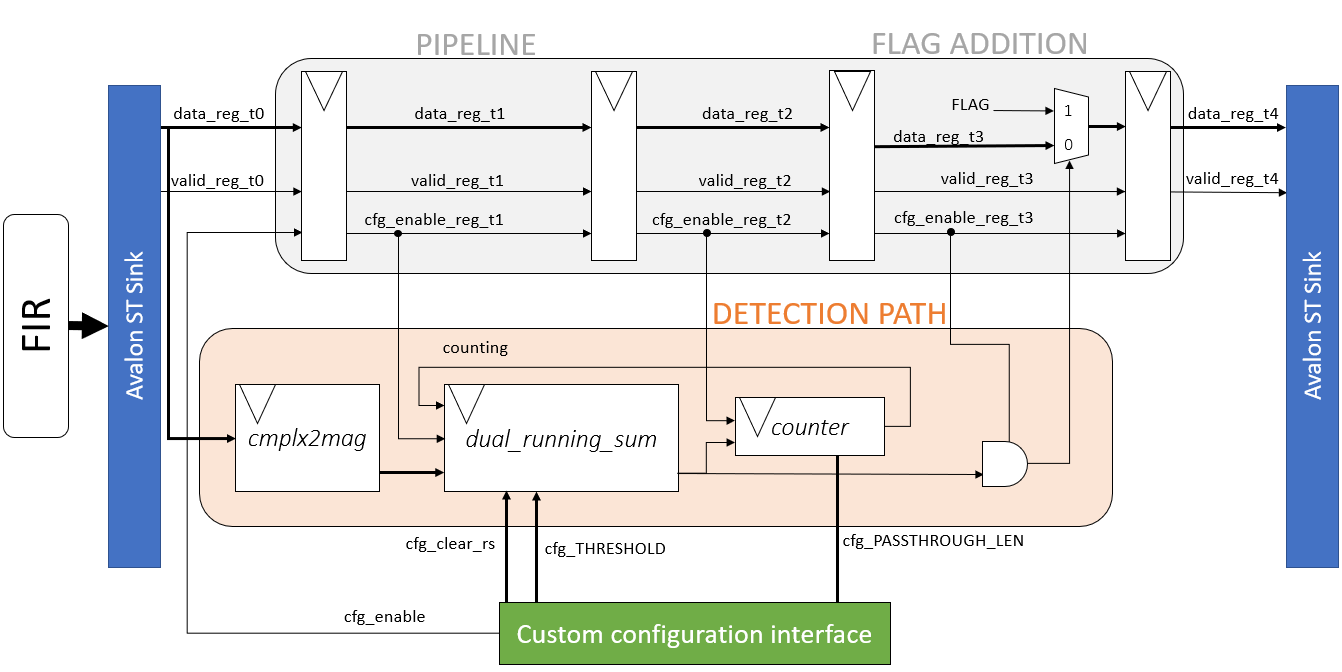
\includegraphics[width=\linewidth]{figures/packet_presence_detection.png}
    \caption{Hardware packet presence detector schematic}
    \label{fig:pd_schematic}
\end{figure}

\subsection{Packet presence detector schematic}
In Figure \ref{fig:pd_schematic} below you can find a schematic of the different modules that compose the PPD. As a reminder, the objective of this block is to add a flag at the start of a packet when a sufficient energy has been detected in the signal. It functions as follows:
\begin{enumerate}
    \item \textbf{Complex to magnitude: } The IQ samples are processed by a \textit{complex to magnitude} block which outputs the magnitude of the complex IQ vector.
    To do so, we calculate the magnitude as the square root of $I^2+Q^2$. As square-root function are difficult to implement in hardware logic, we are thus going to use a very simple and accurate algorithm. The estimate for the first quadrant of the trigonometric circle is drawn on Figure \ref{fig:cmplx2mag}. The mathematical formula is provided to you in Equation \ref{eq:1norm}\footnote{Further information can be found online: \url{https://en.wikipedia.org/wiki/Alpha_max_plus_beta_min_algorithm} and \url{http://dspguru.com/dsp/tricks/magnitude-estimator/}.}.

    \begin{equation}
        |z| = \frac{min(|I|,|Q|)}{4} + max(|I|,|Q|)
        \label{eq:1norm}
    \end{equation}

    \begin{figure}[h]
        \centering
        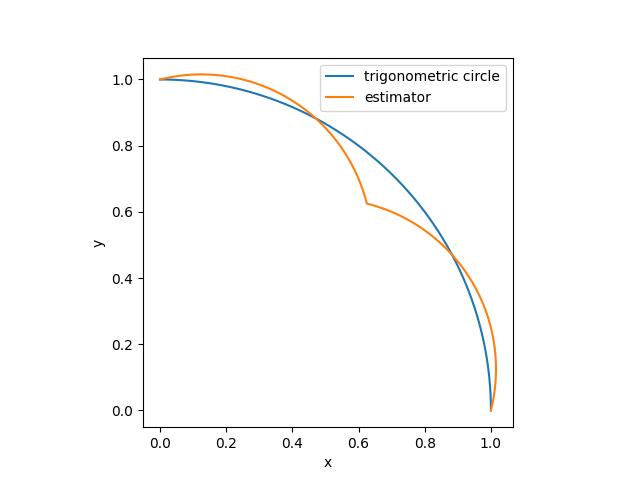
\includegraphics[width=0.45\linewidth]{figures/trigo.png}
        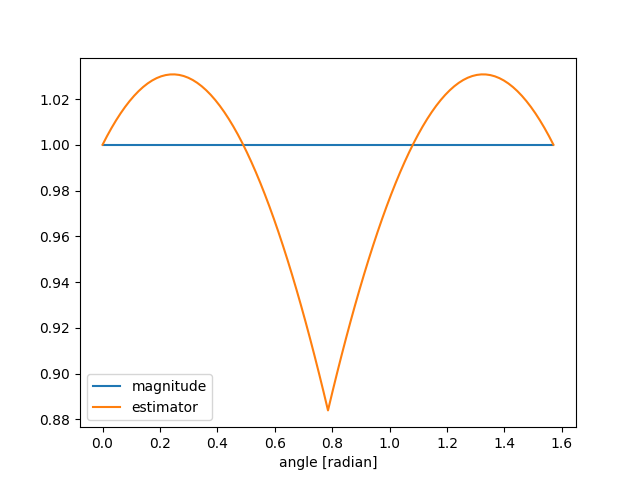
\includegraphics[width=0.45\linewidth]{figures/angle.png}
        \caption{Complex Magnitude Estimator output in x-y coordinates (left) or polar coordinates (right) for input points of the trigonometric circle.}
        \label{fig:cmplx2mag}
    \end{figure}

    \item \textbf{Dual running sum: } The estimated complex magnitude of the samples is then averaged over multiple samples by two moving average filter of different length in series, a short-term sum and long-term one. They are implemented by forwarding input samples in  memory-based \textit{delay lines}, developped by Altera.

    \begin{align}
            y[n] = \sum_{k=0}^{N-1}\left|x[n-k]\right|
    \end{align}

    At each clock cycle an accumulator adds and substracts the first and last magnitude values stored in the delay line to its content. This structure is more efficient than the general FIR because we know each tap is equal to one, we therefore only need two adders.

    \begin{align}
            y[n+1] = y[n] + \left|x[n]\right| - \left|x[n-N+1]\right|
    \end{align}

    The two moving average filters have two different functions. The first one, the short-term sum, receives the sample magnitudes first and its delayed output value are then forwarded to the long-term sum. This longer delay line is used to evaluate the noise power.

    \begin{figure}[h]
        \centering
        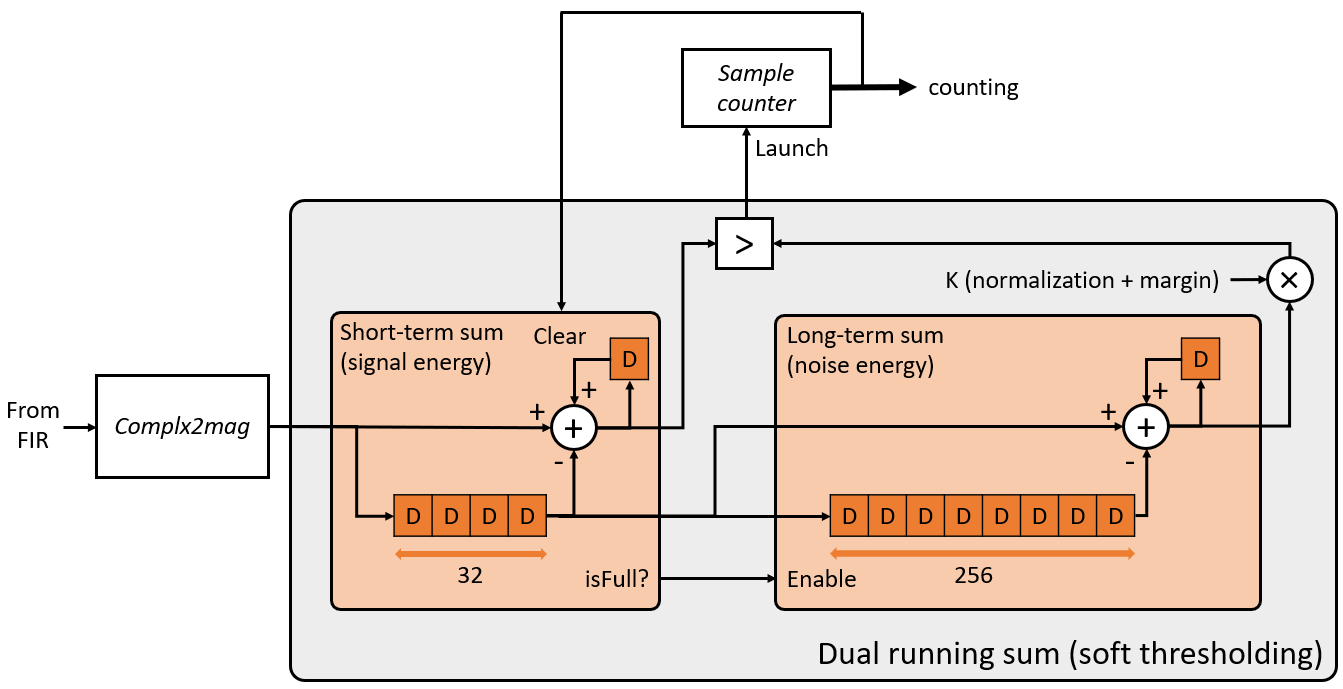
\includegraphics[width=\linewidth]{figures/dual_running_sum_block.png}
        \caption{Architecture of the dual running sum}
        \label{fig:dual_runnign_sum}
    \end{figure}

    The overall architecture of the dual running sum is shown in Fig. \ref{fig:dual_runnign_sum}. If no packet is being received, the samples contain only noise. They pass through the short-term sum and then the long-term one. Both their accumulator can then be seen as noise power estimations.  When a packet arrives, possibly with  higher energy than the noise, the corresponding samples first enter the short-term sum. Its accumulator value therefore increases and might at one point exceed the accumulator value of the long-term sum, which contains only noise samples. At this point, a packet is considered present and a launch signal is triggered.

    To be noted, when a packet is detected and the counter (next block) is enabled, we clear the short-term sum and disable the long-term one, to avoid any retriggering or corruption of our noise evaluation by packet samples.


    \item \textbf{Counter :} This block receives the launch signal of the previous block. This counter block is used to count the samples when the threshold has been reached and avoid triggering a start flag multiple times inside a single packet. During the sequence, a \texttt{running} signal indicates the state of the counter. This signal is used to clear the short-term sum of the dual running sum. The number of samples that are passed is configurable.

    \item \textbf{Flag addition :} A multiplexer is used at the end to replac a sample with a flag, here $I=$\texttt{0x7FF} and $Q=$\texttt{0x7FF}, when the launch signal is triggered.

\end{enumerate}


In order to reduce the length of the critical path between registers, we use a paradigm called \textit{pipelining}. In short, we divide the operations of the PPD into several stages with similar length. As the critical path in this configuration is much shorter, it allows to operate the circuit at a higher frequency. In return, the additional registers add area and energy consumption to the design. It also requires to forward control signals in the pipeline and it can add complexity (see \textit{Control Path} in Figure \ref{fig:pd_schematic}). You will learn the concept of pipelining in details when studying the \textit{pipelined processor} in the course of \texttt{LELEC2531}.

Try to understand the SystemVerilog implementation of those blocks with respect to their theoretical behavior. Pay particular attention to the bus width of intermediate signals, they are computed in order to systematically avoid any overflow of intermediate values!


\subsection{Modification and simulation of the PPD}


We will first ask you to make some modifications to the dual running sum, more specifically to the comparison between the short- and long-term sum results. In order to make it adaptative from GNU Radio, we will use the \texttt{cfg\_THRESHOLD} signal of the packet presence detection module to multiply the result of the long-term sum before comparing it to the short-term sum result. This allows to be more selective regarding the signal-to-noise ratio required to detect the packet. Increasing its value will limit the risk of false alarm due to noise but make your system less sensitive. In short, with this parameter set to 10, the PPD would require a signal magnitude 10 times higher than the noise one to trigger a detection. However, we should also normalize the short-term and long-term result with respect to the delay line length, the second one being here eight times longer than the first. Overall, we ask you to implement the multiplication shown in Figure \ref{fig:dual_runnign_sum}. In the SystemVerilog code, go to the line 199. We ask you to implement both the normalization, i.e. division by eight, and the multiplication operation on the same line. Note that the \texttt{cfg\_THRESHOLD} signal is connected to the \texttt{K} input of the dual running sum module.


\begin{bclogo}[couleur = gray!20, arrondi = 0.2, logo=\bcquestion]{Division by eight}
    \begin{itemize}
        \item Performing multiplications and divisions is much more complex than simple additions. However, when performing operations with values that are power-of-two, things always seem easier. What would be an efficient way to perform the division by eight?
        \item The order in which the two operations are performed, here the multiplication by K and division by eight, would normally have no importance. Is it the case here? Which operation should be performed first and why?
    \end{itemize}
\end{bclogo}

Once you have implemented this function, we should now test the PPD. We have developped a testbench for you, and we will use ModelSim to verify the PPD behavior before deploying it into the complete system. A few python scripts located at \texttt{ip/packet\_presence\_detection/testbench/python} allow you to generate input vectors for the PPD and compare the testbench output with an expected result obtained with python:

\begin{enumerate}
    \item \texttt{1\_input\_gen.py} : generates input vectors and export them as input vector of the PPD HDL implementation.

    \item To generate the testbench, we will use the \textit{Platform Designer}. It allows the interconnection of multiple blocks of a digital design with a more intuitive user interface. Open the \textit{Platform Design} using the shortcut highlighted in Figure \ref{fig:quartus_platform_designer}. Open the \texttt{packet\_presence\_detection\_tb\_gen.qsys}, and go in \textit{Generate} in the upper left corner, then \textit{Generate Testbench System}. Change the path to \texttt{LimeSDR-Mini\_lms7\_lelec210x/ip/packet\_presence\_detection/} and click on \textit{Generate}. To execute the testbench, open ModelSim and change the working directory to\\ \texttt{ip/packet\_presence\_detection/testbench}. Then run \texttt{do run\_sim.tcl} in order to compile and launch the simulation.

\begin{figure}[H]
    \centering
    
\includegraphics[scale=0.7]{figures/quartus_toolbar.PNG}
    \caption{Toolbar of Quartus. The Platform Designer shortcut is highlighted in yellow.}
    \label{fig:quartus_platform_designer}
\end{figure}

    \item \texttt{2\_compare} : when the SystemVerilog testbench has been executed, compares the input data samples to the output of the PPD, plotting them. Is the PPD working as expected? Do not hesitate to ask your questions to a teaching assistant to ensure you fully understand where and why flags are added.
\end{enumerate}

Once you have analysed the results, we will propagate the changes you made to the complete system that will be flashed on the FPGA. Remember we only modified the IP, we now need to propagate those changes to the actual design. In the \textit{Platform Designer}, open the \texttt{lms\_dsp.qsys} design. Nothing has to be done except clicking \textit{"Generate HDL ..."} on the bottom right of the window and update the path to
\texttt{LimeSDR-Mini\_lms7\_lelec210x/lms\_dsp/} if it is not made automatically. Then press on \textit{"Generate"}. The changes you made locally to the PPD have now been propagated. In the Platform Designer, you can quickly observe the structure of the \textit{lms\_dsp} block, with the FIR, the packet presence detection and the different Avalon Streaming Interface.

You can now compile your design and observe the resource and timing report. Be careful when launching a compilation in Quartus, a window may ask you to update the project revision. Answer \textit{"NO"}.

\begin{bclogo}[couleur = gray!20, arrondi = 0.2, logo=\bcattention]{MAX 10 Device Support might not be installed}
    The support for the FPGA device we use might not be installed in the Quartus you have, which will lead to errors in the compilation. The installation instructions are provided in the wiki of the course.

\end{bclogo}

\subsection{Timing and ressource analysis}

As you have seen in course, an important aspect of digital design is to ensure that your design meet both the resource and timing requirements. Indeed, long combinatorial logic path can lead to setup or hold constraints violations. Now that the design has been compiled, you can check the compilation report using the shortcut highlighted in Figure \ref{fig:compilation_report_button}.

\begin{figure}[h]
    \centering
    
\includegraphics[width=\linewidth]{figures/Compilation_report_button.PNG}
    \caption{Toolbar of Quartus. The Compilation Report shortcut is highlighted in red.}
    \label{fig:compilation_report_button}
\end{figure}


In the \textit{"Flow Summary"} tab, the resource utilisation is reported. Observe for instance the number of embedded multipliers that are employed. Moreover, in the \textit{"Analysis \& Synthesis/Timing Analyzer"} tab, you can see the results for the different corners, constraints violations being highlighted in red. Try to identify the faulty clock involved. In the different summary proposed, you can right click on a clock and select \textit{"Report Timing... (In Timing Analyzer UI)"}. In the opened window, just press \textit{"Report Timing"} at the bottom. Those steps are depicted in Figure \ref{fig:report_timing_analyzer}. You can now analyze the most critical path implying the selected clock, as well as the logic cells involved. Try to link the critical path to the RTL design. It should involve a signal starting in the dual running sum module. An easy fix is here to add a register in the path to break in two. This will delay the launch signal by one clock cycle, which is not problematic. \textbf{If you make a modification to the verilog of the PPD, you need to regenerate it in the Platform Designer}.

\begin{figure}[h]
    \centering
    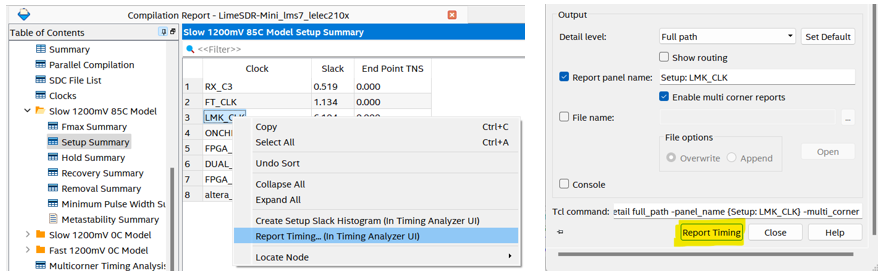
\includegraphics[width=\linewidth]{figures/Report_Timing_Analyzer.png}
    \caption{Steps to analyze the most critical path on a given clock.}
    \label{fig:report_timing_analyzer}
\end{figure}

Moreover, we prevented \textbf{register retiming} which allows the synthesis tool to balance the combinatorial logic across registers when it does not affect the system behaviour. This helps on meeting the timing requirements by offloading parts of long combinatorial path. To enable this setting, go in \textit{"Assignments/Settings/Compiler Settings"} on Quartus and uncheck the \textit{"Prevent register retiming"} box.

Before relaunching a compilation, ask for an assistant to check your modifications, to avoid wasting precious synthesis time. Done? Now relaunch a compilation and analyze the results. Again, if a window asks you to update the project revision, answer \textit{"NO"}. Is there still a timing constraint violation? Can you still link the most critical path to the HDL design?

To analyse the ressource used by the design, you can look at the \textit{Hierarchy} tab in the \textit{Project Navigator}. More than navigating through the design, you can also look at the ressource used by each module. Analyse the resource usage of the PPD, more specifically the memory bits and the DSP.
\begin{comment}
\subsection{From Euclidean norm to Absolute-value norm}

In order to meet the timing requirements, another solution is to use a less complex estimation of the IQ samples magnitude. We are thus going to use a very simple and accurate algorithm that does not have the burden of implementing the complex logic of \textit{integer multiplication}. The estimate for the first quadrant of the trigonometric circle is drawn on Figure \ref{fig:cmplx2mag}. We ask you to implement it in System Verilog, the mathematical formula being provided to you in Equation \ref{eq:1norm}\footnote{Further information can be found online: \url{https://en.wikipedia.org/wiki/Alpha_max_plus_beta_min_algorithm} and \url{http://dspguru.com/dsp/tricks/magnitude-estimator/}.}. Your modification of the \texttt{cmplx2mag} module must be done in the \texttt{USER CODE} parts, which goes from line 45 to 52 and on line 210. As we were performing two multiplications and one addition in the previous algorithm ($I^2+Q^2$), the data bus at the output of the \textit{cmplx2mag} module was specified as twice the input data bit width (due to multiplication) plus one (due to the addition). This is specified on line 210, do not forget to adapt it for the new algorithm. In the next step, you are going to make a behavioral simulation of you implementation to validate it.

\begin{equation}
    |z| = \frac{min(|I|,|Q|)}{4} + max(|I|,|Q|)
    \label{eq:1norm}
\end{equation}

\begin{figure}[h]
    \centering
    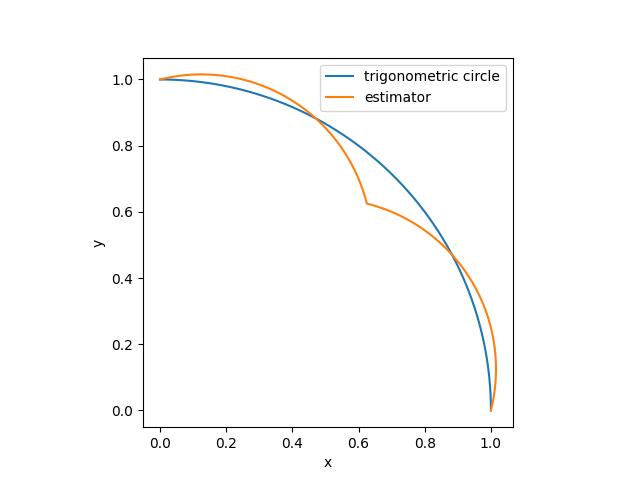
\includegraphics[width=0.45\linewidth]{figures/trigo.png}
    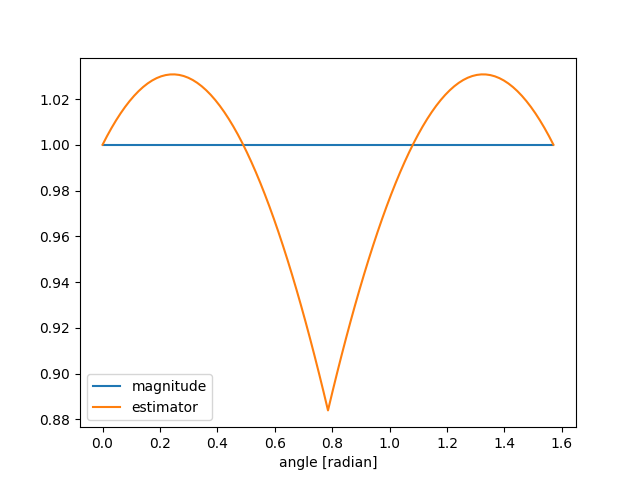
\includegraphics[width=0.45\linewidth]{figures/angle.png}
    \caption{Complex Magnitude Estimator output in x-y coordinates (left) or polar coordinates (right) for input points of the trigonometric circle.}
    \label{fig:cmplx2mag}
\end{figure}


Now that you have a functional design for the PPD with the Absolute-value norm, we can perform a synthesis of the complete design. Do not forget to propagate your change by regenerating the HDL via the Platform Designer. Observe the resource usage and the timing report, is there still a timing constraint violation?

\end{comment}

%%\section{Demodulating a capture with GNU Radio}

The teaching team recorded a capture containing five packets sent with the S2LP radio.
As a first introduction to GNU Radio, you will demodulate this capture using the 2-FSK demodulator and CFO estimators you wrote in the previous hands-on.

\subsection{Installing the \texttt{gr-fsk} module}

For this session, we provide you a version of the project that includes both a full software implementation for the MCU and a GNU Radio
module compatible with the S2LP radio. Download this project on Moodle and unzip it.

GNU Radio provides many built-in digital signal processing blocks (similarly to LabView), however these blocks are not sufficient to implement a functional FSK receiver.
The teaching team hence developed a new \href{https://wiki.gnuradio.org/index.php/OutOfTreeModules}{out-of-tree module} named
\texttt{gr-fsk} that contains all the blocks (preamble detection, synchronization, demodulation, packet parser, ...) needed to build an entire receiver chain for the S2LP radio.
Before running GNU Radio, this module must be compiled and installed. To this end, open a terminal, go into the \texttt{telecom/sdr/gr-fsk} folder and execute the following commands:

\begin{bash}
    mkdir build
    cd build/
    cmake ..
    sudo make install
    sudo ldconfig
\end{bash}
The module is now installed.

To ensure GNU Radio will be able to locate the installation directory of this custom package, we need to check the \texttt{PYTHONPATH} environment variable of GNU Radio. In the prompted log of the above installation commands, you should see multiple lines such as \texttt{/usr/local/XXX/dist-packages/fsk/XXX}. Now run the command :


\begin{bash}
echo $PYTHONPATH
\end{bash}

If the path from the compilation log (up to \texttt{dist-packages}) does not appear, we will need to add it to the \texttt{PYTHONPATH} variable with the following command you should adapt to your case :


\begin{bash}
echo "export PYTHONPATH='/usr/local/XXX/dist-packages/:$PYTHONPATH'" >> ~/.bashrc
\end{bash}

\subsection{Running the GNU Radio Companion}

GNU Radio may either be used directly using Python scripts or through a GUI software named GNU Radio Companion. It is much more convenient to use the latter to design and experiment receiver chains.
Start the GNU Radio Companion (\textit{``Programming -> GNU Radio Companion''}) and open the application \texttt{gr-fsk/apps/decode\_capture.grc}.
This application reads a prerecorded capture from a file
and demodulates it using the FSK receiver architecture that has been explained in the simulation hands-on. The operations carried out by the different blocks are exactly identical to those of the simulation framework we provided you.

\begin{bclogo}[couleur = gray!20, arrondi = 0.2, logo=\bcinfo]{GNU Radio parameter adjustement}
    In the GNU Radio GUI, the low-pass filter might be highlighted in red due to an error depending on the Ubuntu release you are using. Double-click on it and on the part highlighted in red and select the corresponding one. (Normally the error, if present, is on the \textit{Window} parameter which should be set to \textit{Hamming})
\end{bclogo}

\begin{figure}[H]
    \centering
    
\includegraphics[scale=1]{figures/buttons.PNG}
    \caption{GNU Radio buttons to generate the Python script, running and stopping the application.}
    \label{fig:buttons}
\end{figure}
\texttt{.grc} files are designs which can be graphically edited in the companion, but they cannot directly be executed.
Instead, the companion generates Python scripts based on the \texttt{.grc} design. To generate the corresponding script, press the second button starting from the left (i.e., the one with a box and an arrow) shown in Fig.~\ref{fig:buttons}.
The generated script can then be executed by pressing the \textit{Run} button (third button starting from the left).

\begin{bclogo}[couleur = gray!20, arrondi = 0.2, logo=\bcinfo]{Setting the path of the \textit{File Source}}
    You may need to fix the path of capture in the block \textit{File Source}.
    The capture is located at \texttt{gr-fsk/misc/fsk\_capture.mat}.
    After modifying the design in the companion, re-generate the corresponding Python script before launching the application.
\end{bclogo}

When running the application, the console on the bottom left corner on the screen indicates the events processed by the different blocks.
Since both the estimation of the CFO and the demodulation functions are not implemented in this version of the project,
you should observe that 5 packets are detected with a CFO of \SI{0}{\hertz} and are incorrectly demodulated (all payload bytes are demodulated to zeroes).

\subsection{Modifying the \texttt{gr-fsk} module}

To correctly demodulate the capture, you now need to plug in the demodulator and CFO estimator from the previous hands-on into the \texttt{gr-fsk} module.
The \texttt{gr-fsk} blocks are written in Python and are all located in the folder \texttt{gr-fsk/python}.
Open the file \texttt{gr-fsk/python/demodulation.py}, which implements the \textit{Demodulation} block. For all \texttt{gr-fsk} blocks, the teaching team wrote the boilerplate code that
handles the buffers inside GNU Radio. On the contrary, the operations that are specific to the signal processing (e.g., demodulation, estimating the CFO or STO, ...) have been outsourced
to external functions. These functions have almost similar prototypes to the corresponding functions of the simulation framework.
\textbf{You may hence validate your signal processing functions in the simulation framework before inserting them in GNU Radio.}

\begin{bclogo}[couleur = gray!20, arrondi = 0.2, logo=\bcinfo]{Remark on writing code that is \textit{fast enough}}
    In the simulation framework, your code did not have to be fast to work.
    \textbf{For the measurements}, however, the code should run in \textit{real-time},
    meaning that, if your code is too slow, the packet will arrive faster
    than they are decoded, eventually leading to errors.

    If your code did work in the simulation tests, but not in GNU Radio, please
    be careful to avoid too many for-loops, and prefer using array operations
    directly.

    You can use the \texttt{timeit} Python decorator from
    \texttt{gr-fsk/python/utils} to measure how much time each function takes,
    and identify the ones that are important to optimize.
\end{bclogo}

Nonetheless, it is important that you gain some understanding of how custom GNU Radio blocks are written.
Please take some time to dive into \texttt{demodulation.py}. The functions \texttt{\_\_init\_\_} (initialization of the block with the specified parameters),
\texttt{forecast} (indicates to GNU Radio how many input samples are needed to provide $N$ output samples) and \texttt{general\_work} (actual function that performs the processing) are common to all GNU Radio blocks.
The companion however does not directly read the Python files to understand how a block is implemented. Instead, each block comes with a
YAML file, read by the companion, which includes all the information required by the tool: types of the input and output signals, parameters,
callback functions, ... Open the file \texttt{gr-fsk/grc/fsk\_demodulation.block.yml} and browse it also.

Once you went over the Python and YAML files, put the demodulation function you wrote for the previous hands-on in the external \texttt{demodulate} function. Repeat the same procedure for the CFO estimation in the function
\texttt{cfo\_estimation} of \texttt{gr-fsk/python/synchronization.py}. Then, before running the GNU Radio application again, you need to re-do an installation to propagate your changes:

\begin{bash}
    cd build/
    sudo make install
\end{bash}

\begin{bclogo}[couleur = gray!20, arrondi = 0.2, logo=\bcinfo]{Usage of the build folder}
    Creating and populating the build directory with \texttt{cmake} needs only to be done once.
    Afterwards it is sufficient to only do an install to propagate your changes in the Python files to the system.
\end{bclogo}

After the installation of your modifications, re-launch the application.
If the two functions \texttt{demodulate} and \texttt{cfo\_estimation} are correctly implemented, you should now observe that all 5 packets are rightly demodulated (with the payload bytes increasing succesively from 0 to 99)
and that the CFO of each packet is approximately located around \SI{7800}{\hertz}.

\section{Live demodulation with a cable}

Now that the \texttt{gr-fsk} blocks are fully functional, the next step consists in receiving and demodulating in real-time packets from the MCU.
The project contains a full MCU software implementation with a driver to interact with the S2LP radio.
This software features an evaluation mode of the radio that transmits several packets in a row with different transmit (Tx) output power levels.
To verify the entire chain (Tx and Rx) at a very high signal-to-noise ratio (SNR), we first use an SMA cable to connect the S2LP radio and the LimeSDR Mini.
The reference datasheet of the radio is available at the following link: \href{https://www.st.com/resource/en/datasheet/s2-lp.pdf}{\textcolor{blue}{[S2-LP datasheet]}}.

\subsection{Preparing the setup}

\begin{enumerate}
    \item Connect the S2LP radio on the MCU to the Rx port of the LimeSDR Mini board using the SMA cable.
    \item Connect the Nucleo board to your computer.
    \item Connect the LimeSDR Mini board to your computer using the extension USB cable.
    To avoid any performance loss, do not connect the LimeSDR Mini board directly to your computer, as interference from your computer may corrupt the received signal.
    \item If on VirtualBox, pass both devices to the guest system (\textit{"Devices -> USB -> ..."}). On WSL, see install guidelines how to attach the LimeSDR.
\end{enumerate}

%\begin{bclogo}[couleur = gray!20, arrondi = 0.2, logo=\bcinfo]{Passing the LimeSDR Mini to the VM}
%    Depending on your computer, you may have difficulties to pass the LimeSDR Mini to the guest system.
%    When passing the devices in the VirtualBox menu, use the command \texttt{lsusb} in a terminal to verify if the device has correctly been passed.
%    If you are unable to pass the board after a few trials, shutdown the VM, \textbf{close the VirtualBox manager and restart it}, and relaunch the VM.
%\end{bclogo}

\subsection{Setting up the MCU}

Open the MCU software project \texttt{mcu} with Eclipse (\textit{"File -> Open projects from file system ..."}).
In the configuration file \texttt{Core/Inc/config.h}, ensure that the following macros are defined as
\begin{itemize}
    \item \texttt{ENABLE\_RADIO 1}: initialize the S2LP radio when booting.
    \item \texttt{RUN\_CONFIG EVAL\_RADIO}: use the radio evaluation mode.
    \item \texttt{ENABLE\_UART 1}: enable the UART.
    \item \texttt{DEBUGP 1}: enable the debug prints.
\end{itemize}

Beside the general configuration file, the parameters of the radio evaluation mode are defined in \texttt{Core/Inc/eval\_radio.h}.
Open this file and try to understand the different parameters.

Afterwards, compile the software and flash the Nucleo board. Open a serial console to \texttt{/dev/ttyACM0} and press the button B1 to start transmitting packets.

\begin{bclogo}[couleur = gray!20, arrondi = 0.2, logo=\bcinfo]{MCU build error}
    If you encounter an error when building the MCU software project, this is probably because you need to update the project settings. To do so, please open the \texttt{ioc} and click \textit{Yes} when prompted to migrate the project to the new version. After, \textbf{do not forget} to re-generate. Finally, you should be able to compile the project. Some errors about \texttt{\_getpid} and \texttt{\_kill} may be left, but you can safely ignore them.
\end{bclogo}

\subsection{Running the GNU Radio application}

The teaching team prepared a GNU Radio application ready to receive packets from the S2LP radio.
Open the application \texttt{gr-fsk/apps/eval\_limesdr.grc}. Instead of reading a stream from a file, the application uses the LimeSDR Mini
to retrieve samples. Try to understand the effects of the following variables in the application:
\begin{itemize}
    \item \texttt{packet\_len}: length of the packet, in bytes.
    \item \texttt{rx\_gain}: gain of the amplification stage in the receiver chain, in decibels. It can be change during operation using a slider.
    \item \texttt{detect\_threshold\_entry}: threshold of the preamble detection. You can also change it during operation using a slider.\\
    Open the Python file \texttt{gr-fsk/python/preamble\_detection.py} to understand its behavior.
    \item The cut-off frequency and transition width of the low pass filter.
\end{itemize}

If the role of some of these parameters are unclear to you, please ask the assistant for clarifications.
Moreover, to allow the calculation of the SNR and the related $\boldsymbol{\sfrac{\varepsilon}{N_0}}$, the \textit{Noise estimation on query} can be activated during operation through the GUI by pressing the button. It computes the noise power $K$ times over $M$ samples. When a packet is received, the \textit{Synchronization}  block computes the signal power and uses the noise power evaluation previously made to evaluate the $\boldsymbol{\sfrac{\varepsilon}{N_0}}$. Be sure to evaluate the noise power before you enable the chain with the \textit{Enable chain} check box, or when you change the receiver gain. We advice you to look at Section~\ref{sec:appendix} to understand the mathematical derivation of the $\boldsymbol{\sfrac{\varepsilon}{N_0}}$ estimation.

\begin{bclogo}[couleur = gray!20, arrondi = 0.2, logo=\bcinfo]{Usage of the build folder}
    In the GNU Radio GUI, the low pass filter initially appear gray. This indicates the block is currently disabled. You can easily enable or disable a block by selecting it and pressing E or B respectively. Do not forget to route the signal accordingly.
\end{bclogo}


When launching the GNU Radio application, the procedure is the following:
\begin{enumerate}
    \item Launch the GNU Radio application.
    \item Perform a noise estimation by clicking on \textit{"Noise estimation query"}.
    \item Update the detection threshold based on the estimated noise standard deviation.
    \item Enable the chain by checking the box \textit{Enable chain}.
    \item Start transmitting packets with the MCU.
\end{enumerate}

To be noted, there is \textit{TX power} variable that can be changed but it will only be useful later on in the project when you will make BER measurements.

\begin{bclogo}[couleur = gray!20, arrondi = 0.2, logo=\bcinfo]{Help, my virtual machine becomes unstable or freezes!}
    If you observe that your virtual machine is unable to smoothly run the GNU Radio application, you may need to increase the number
    of CPU cores and the memory shared with the VM.
\end{bclogo}

\subsection{Optional: Recording a capture}

When debugging GNU Radio blocks, recording a capture is a very useful technique to run the same experiment again in identical conditions.
An application which performs a recording of the samples acquired by the LimeSDR Mini is provided in \texttt{gr-fsk/apps/record\_capture.grc}.
Try to use this application to record a new capture while the MCU transmits packets, and then demodulate it using \texttt{gr-fsk/apps/decode\_capture.grc}.

\section{Live demodulation over the air}

In the ecomonitoring application, the MCU needs to communicate with the gateway over the air, and not using a cable.
The final part of this hands-on session consists in using the antennas to transmit and receive the packets.

\subsection{Frequency allocation}

Since all wireless transmissions use the same medium (i.e., the air), it is important that each group uses a different carrier frequency to avoid interfering with other groups.
To this end, please use the following frequency allocation scheme, in which each group is allocated a bandwidth of \SI{2}{\mega\hertz}:
\begin{table}[h]
    \centering
    \begin{tabular}{c|c}
        Group number & Allocated carrier frequency\\
        \hline
        Group A & \SI{860}{\mega\hertz}\\
         Group B & \SI{862}{\mega\hertz}\\
         Group C & \SI{864}{\mega\hertz}\\
         ... & ...
    \end{tabular}
    \caption{Frequency allocation scheme among the groups.}
    \label{tab:freq_alloc}
\end{table}

The allocated carrier frequency must be configured both in the MCU and in the GNU Radio Companion.
\begin{itemize}
    \item In the MCU code, open the file \texttt{Core/Inc/s2lp.h} which contains the parameters used by the radio.
    Try to understand the different parameters and modify the macro \texttt{BASE\_FREQ} to your allocated carrier frequency.
    \item In GNU Radio, modify the variable \texttt{carrier\_freq}.
\end{itemize}
For more details on the different parameters and modes in which the S2LP radio can be configured to, have a look at Tables 12 (page 13) and 40 (page 28) in the S2-LP datasheet.

\subsection{Running the GNU Radio application}

Once the carriers are correctly configured, replace the SMA cable with the antennas and run the application.
Since transmitting over the air implies that the signal at the receiver will have a much weaker power compared to a transmission over a cable,
it is necessary to increase the Rx gain in the LimeSDR Mini. This can be done using the GUI when the application is running. \textbf{Run the application and set the gain at \SI{60}{\decibel}.}
You should now be able to receive packets over the air.
You might need to try several distances (between 1 and 5 meters) and different values of the variable \texttt{detect\_threshold} to achieve a functional communication.

\subsection{Measuring the noise level}
\label{sec:appendix}

To estimate $\boldsymbol{\sfrac{\varepsilon}{N_0}}$ in measurement, we first estimate the SNR based on the symbol power $P_S$ and the noise power $P_N$. The noise power can be evaluated by computing the variance of the received signal when no packet is transmitted,  $\sigma_w^2$. To compute $P_S$, we evaluate the signal variance  when a packet is received, $\sigma_p^2$, and remove the noise contribution. Thereby, the SNR is computed as
\begin{equation}
    \textrm{SNR} = \frac{P_S}{P_N} = \frac{\sigma_p^2 - \sigma_w^2}{\sigma_w^2}.
\end{equation}
We can now derive $\boldsymbol{\sfrac{\varepsilon}{N_0}}$ by expressing $P_N$ based on the noise bandwidth which is equal to $B*R_{RX}$ prior to the low-pass filter. On the other hand, $P_S$ can be written with respect to the symbol energy $\varepsilon$ and its duration $\sfrac{1}{B}$. We thereby obtain the expression
\begin{equation}
    \frac{P_S}{P_N} = \frac{\varepsilon B}{N_0 B R_{RX}} = \frac{\varepsilon}{N_0 R_{RX}} \leftrightarrow \frac{\varepsilon}{N_0} = R_{RX}\textrm{SNR}.
\end{equation}
In practice, an estimate of the noise power $\sigma_w^2$ can be obtained using the \textit{"Noise estimation query"} block during operation. Several estimation of $\sigma_w^2$ are made and their mean is calculated.

%%<<<<<<< refs/remotes/upstream/main
\section{To go further : configuration signal exchanges between FPGA and GNU Radio}

=======
>>>>>>> Revert "enlever le chain de argu"
\subsection{SystemVerilog parameters}
When instantiating the IP in the subsystem, you are allowed to define the values of a few \textit{SystemVerilog parameters} for the top-level module of the preamble detector, as shown in Figure \ref{fig:pd_hard_param}. Those parameters described in the Table \ref{table:pd_hard_param}.

\begin{figure}[!h]
    \centering
<<<<<<< refs/remotes/upstream/main
    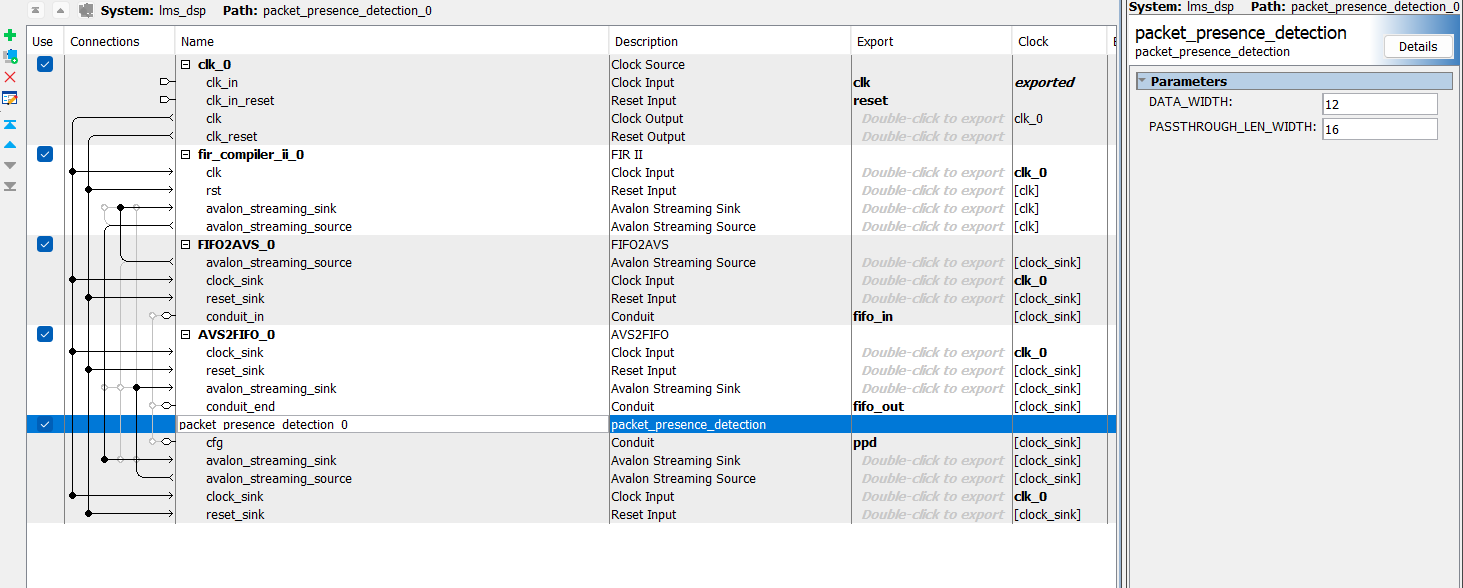
\includegraphics[width=\linewidth]{figures/ppd_detect_qsys_config.PNG}
    \caption{SystemVerilog parameters of the packet presence detector in QSYS.}
=======
    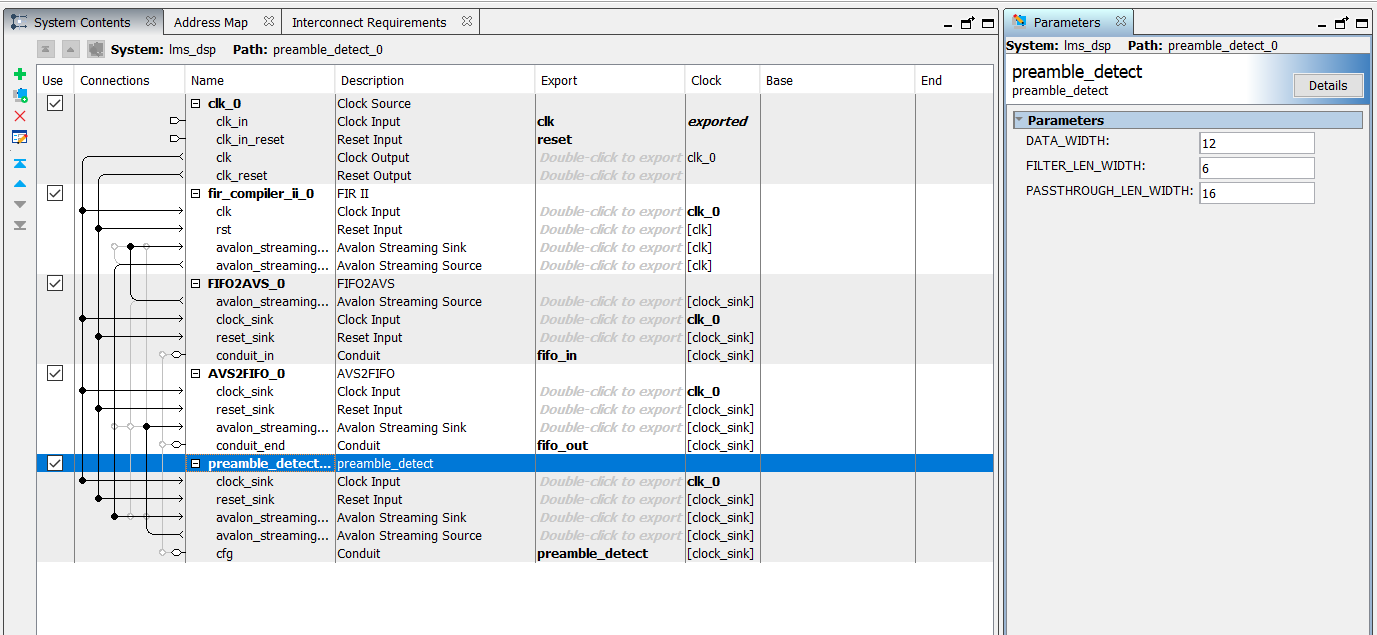
\includegraphics[width=\linewidth]{figures/preamble_detect_qsys_config.PNG}
    \caption{SystemVerilog parameters of the preamble detector in QSYS.}
>>>>>>> Revert "enlever le chain de argu"
    \label{fig:pd_hard_param}
\end{figure}

\begin{table}[!h]
\centering
\begin{tabular}{|p{0.36\linewidth}|p{0.48\linewidth}|p{0.08\linewidth}|}
\hline
Parameter & Description & Default value \\
\hline
\textsc{DATA\_WIDTH} & Bit width of the samples & 12 \\
\hline
<<<<<<< refs/remotes/upstream/main
=======
\textsc{FILTER\_LEN\_WIDTH} & Bit width of the configurable moving average filter length & 6 \\
\hline
>>>>>>> Revert "enlever le chain de argu"
\textsc{PASSTHROUGH\_LEN\_WIDTH} & Bit width of the configurable number of samples to pass-through once the threshold is reached & 16 \\
\hline
\end{tabular}
\caption{SystemVerilog parameters of the \texttt{preamble\_detector} IP}
\label{table:pd_hard_param}
\end{table}

\subsection{Configuration signals}
\begin{sloppypar}
<<<<<<< refs/remotes/upstream/main
Additionally, there are several configuration signals that can be changed during operation from GNU Radio for better flexibility. Those configuration signals are listed in Table \ref{table:pd_soft_param}, you can trace them in the VHDL code, they are coming from the \texttt{fpgacfg} module defined in \texttt{LimeSDR-Mini\_lms7\_lelec210x/src/spi/fpgacfg.vhd} and located in the design hierarchy at \texttt{lms7\_trx\_top/inst0\_nios\_cpu/cfg\_top\_inst1/fpgacfg\_inst0}, as shown in Figure \ref{fig:design_hier_fpgacfg}.
=======
Additionally, there are several configuration signals that can be changed during operation from GNU Radio for better flexibility. Those configuration signals are listed in Table \ref{table:pd_soft_param}, you can trace them in the VHDL code, they are coming from the \texttt{fpgacfg} module defined in \texttt{LimeSDR-Mini\_lms7\_lelec210x/src/spi/fpgacfg.vhd}and located in the design hierarchy at \texttt{lms7\_trx\_top/inst0\_nios\_cpu/cfg\_top\_inst1/fpgacfg\_inst0}, as shown in Figure \ref{fig:design_hier_fpgacfg}.
>>>>>>> Revert "enlever le chain de argu"
\end{sloppypar}

This module contains a RAM with 16-bit words that retains the configuration of various elements of the FPGA. We used available addresses to put our custom configuration, the address map is written in the repo README. There are default values assigned at reset for the memory bits (Figure \ref{fig:design_hier_fpgacfg}) but they can be changed with a write operation.

\begin{table}[!h]
\centering
\begin{tabular}{|p{0.22\linewidth}|p{0.25\linewidth}|p{0.34\linewidth}|p{0.08\linewidth}|}
\hline
Configuration signal & Description & Allowed values\\
\hline
<<<<<<< refs/remotes/upstream/main
\texttt{cfg\_enable} & Enable or disable the PPD. & $\left\{0,1\right\}$ \\
\hline
\texttt{cfg\_clear\_} & Clear the delay lines of the dual running sum. & $\left\{0,1\right\}$ \\
\hline
\texttt{cfg\_PASSTHROUGH\_LEN} & Number of samples to pass-through after a start flag has been added. Avoid any retriggering of this flag meanwhile. & $\left[1,2^{\textsc{PASSTHROUGH\_LEN\_WIDTH}}-1\right]$ \\
\hline
\texttt{cfg\_THRESHOLD} & Value to multiply the normalized result of the long-term sum, before comparison. & $\left[1,2^{8}-1\right]$ \\
\hline
\end{tabular}
\caption{Configuration signals \texttt{packet\_presence\_detection} IP}
=======
\texttt{cfg\_enable} & Enable or disable the preamble detector. When disabled, the samples are always passing through. & $\left\{0,1\right\}$ \\
\hline
\texttt{cfg\_FILTER\_LEN} & Size of the moving average filter. & $\left[1,2^{\textsc{FILTER\_LEN\_WIDTH}}-1\right]$ \\
\hline
\texttt{cfg\_PASSTHROUGH\_LEN} & Number of samples to pass-through once the threshold is reached. & $\left[1,2^{\textsc{PASSTHROUGH\_LEN\_WIDTH}}-1\right]$ \\
\hline
\texttt{cfg\_THRESHOLD} & Value to be compared with the moving average filter output. & $\left[1,2^{32}-1\right]$ \\
\hline
\end{tabular}
\caption{Configuration signals \texttt{preamble\_detector} IP}
>>>>>>> Revert "enlever le chain de argu"
\label{table:pd_soft_param}
\end{table}

\begin{figure}[!h]
    \centering
    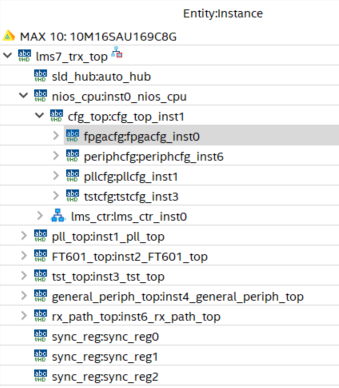
\includegraphics[width=0.3\linewidth]{figures/design_hierarchy_fpgacfg.PNG}
    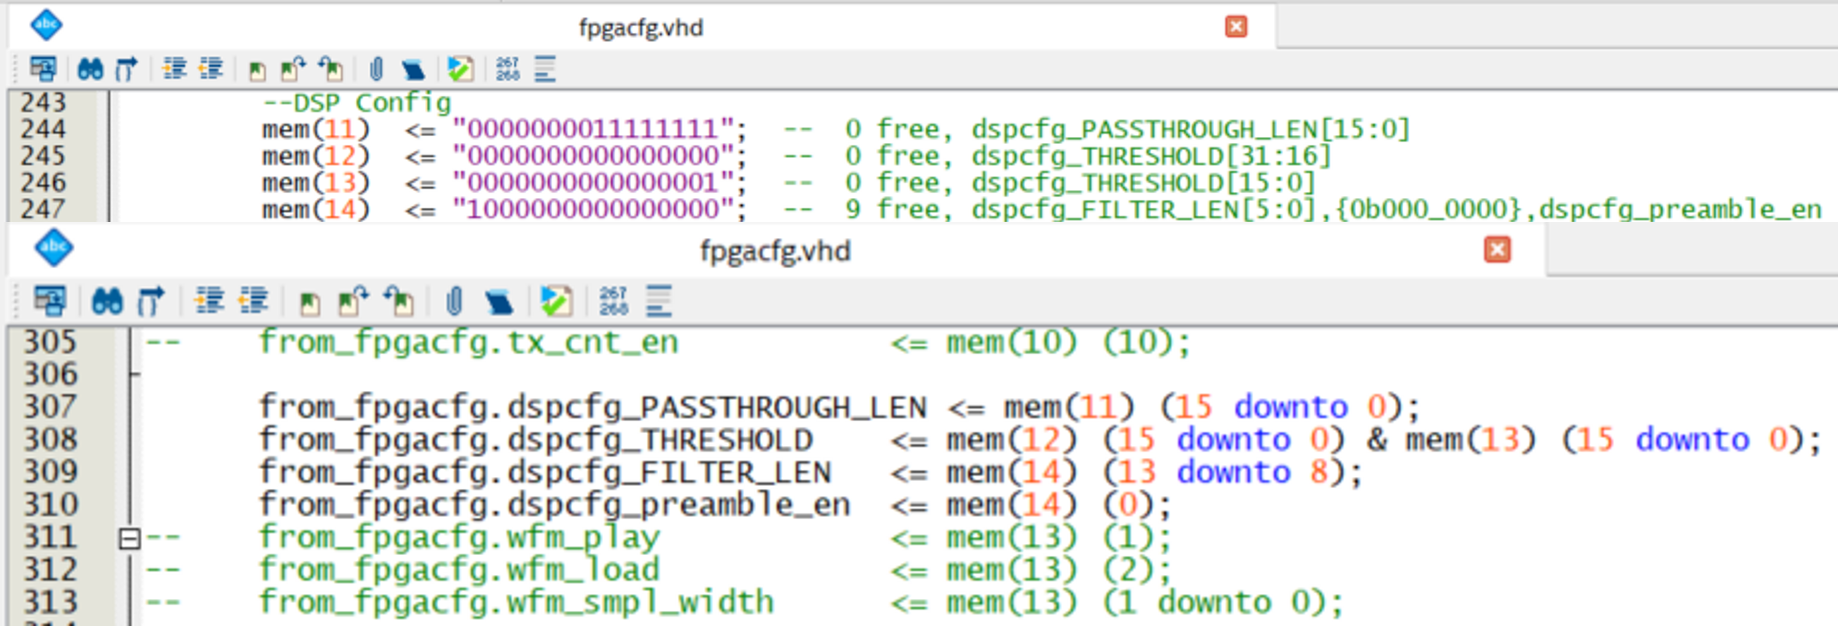
\includegraphics[width=0.6\linewidth]{figures/design_hierarchy_fpgacfg_both.PNG}
    \caption{Configuration signal location in the design hierarchy (left). Assignment and reset values for the DSP configuration signals (right).}
    \label{fig:design_hier_fpgacfg}
\end{figure}

\subsubsection{Read/write operations of the configuration signals from GNU Radio}
The GNU Radio block of the LimeSDR-Mini uses a C++ library called \textit{LimeSuite} in order to write data to the FPGA configuration memory. In the following paragraph, the configuration flow inside LimeSuite and the hardware is briefly described.

\begin{sloppypar}
\paragraph{gr-limesdr GUI interface}
In our custom version of the limeSDR GNU Radio block, we added fields to configure the hardware preamble detector. To do so, we modified the file \texttt{gr-limesdr/grc/limesdr\_fpga\_source.block.yml} and added a GUI callback function named \texttt{set\_dspcfg\_preamble}. This function is in turn defined in \texttt{gr-limesdr/lib/source\_impl.cc} and \texttt{gr-limesdr/lib/device\_handler.cc}. Please take a look at the end of \texttt{device\_handler.cc} and understand the functions we added. At the core of all of them, we use \texttt{modify\_spi\_reg\_bits}, shown in Figure \ref{fig:modify_spi_reg_bits}, that uses LimeSuite \texttt{LMS\_WriteFPGAReg} function. Pay attention to the arguments and try to make the link with the configuration memory of the FPGA, the input structures are defined in \texttt{gr-limesdr/lib/fpga\_register\_map.h}.
\end{sloppypar}

\begin{figure}[!h]
    \centering
    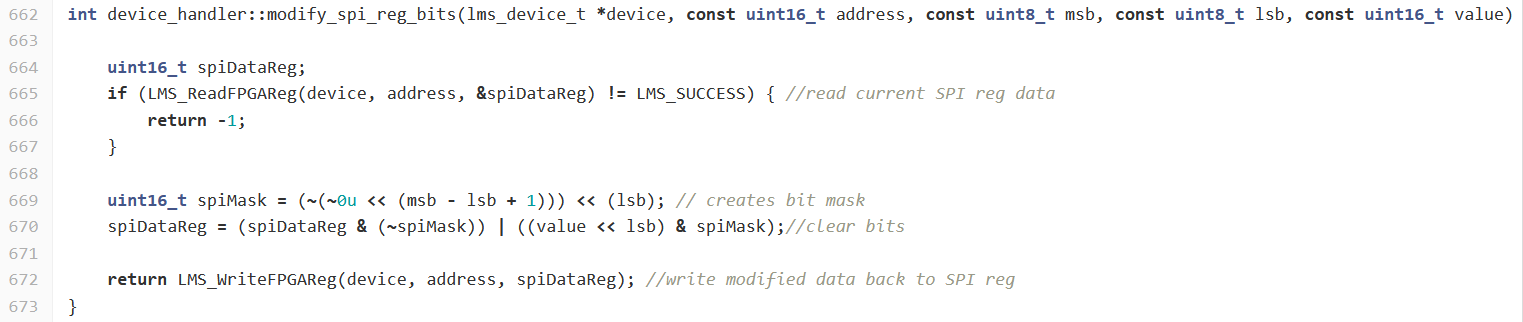
\includegraphics[width=\linewidth]{figures/grlimesdr_write_fpgacfg.PNG}
    \caption{Software interface between GNU Radio and LimeSuite.}
    \label{fig:modify_spi_reg_bits}
\end{figure}

\paragraph{NIOS Interface}
When calling \texttt{LMS\_WriteFPGAReg}, the functions wrap the address and value of the register we wish to configure inside a packet that is transmitted through USB. The complete callstack inside the library is described in the repo README. The USB interface is connected to an FTDI Chip which is in turn interfaced with the FPGA, as shown in Figure \ref{fig:limesdr_mini_schematic}.

Inside the FPGA, we have:
\begin{enumerate}
    \item An FTDI arbitrer that decodes a first part of the packet header to forward it through a configuration FIFO (\texttt{EP02\_fifo}) towards the NIOS subsystem. This arbitration is necessary as we have two other FIFOs coming from the NIOS subsystem and the RX data path (\texttt{EP83\_fifo} and \texttt{EP82\_fifo} respectively).
    \item A NIOS Softcore processor instantiated inside the FPGA reads the FIFO and decodes the second part of the packet header, it then forwards the packet data to through an SPI Master.
    \item An SPI Slave is connected with the configuration memory and writes the received data at the correct address.
\end{enumerate}

\begin{bclogo}[couleur = gray!20, arrondi = 0.2, logo=\bcinfo]{Additional resources}
To help you understand this complex path, we provided you with resources you can find on moodle or \texttt{LimeSDR-Mini\_lms7\_lelec210x/doc/} folder. The file \texttt{FPGA\_config\_path.pdf} with annotations referring to the above paragraph should be helpful, several elements have been hidden to ease the reading. You can also use freely the RTL viewer to skim through the design hierarchy graphically instead of opening files, see Figure \ref{fig:rtl_viewer} for further details.
\end{bclogo}

\begin{figure}[!h]
    \centering
    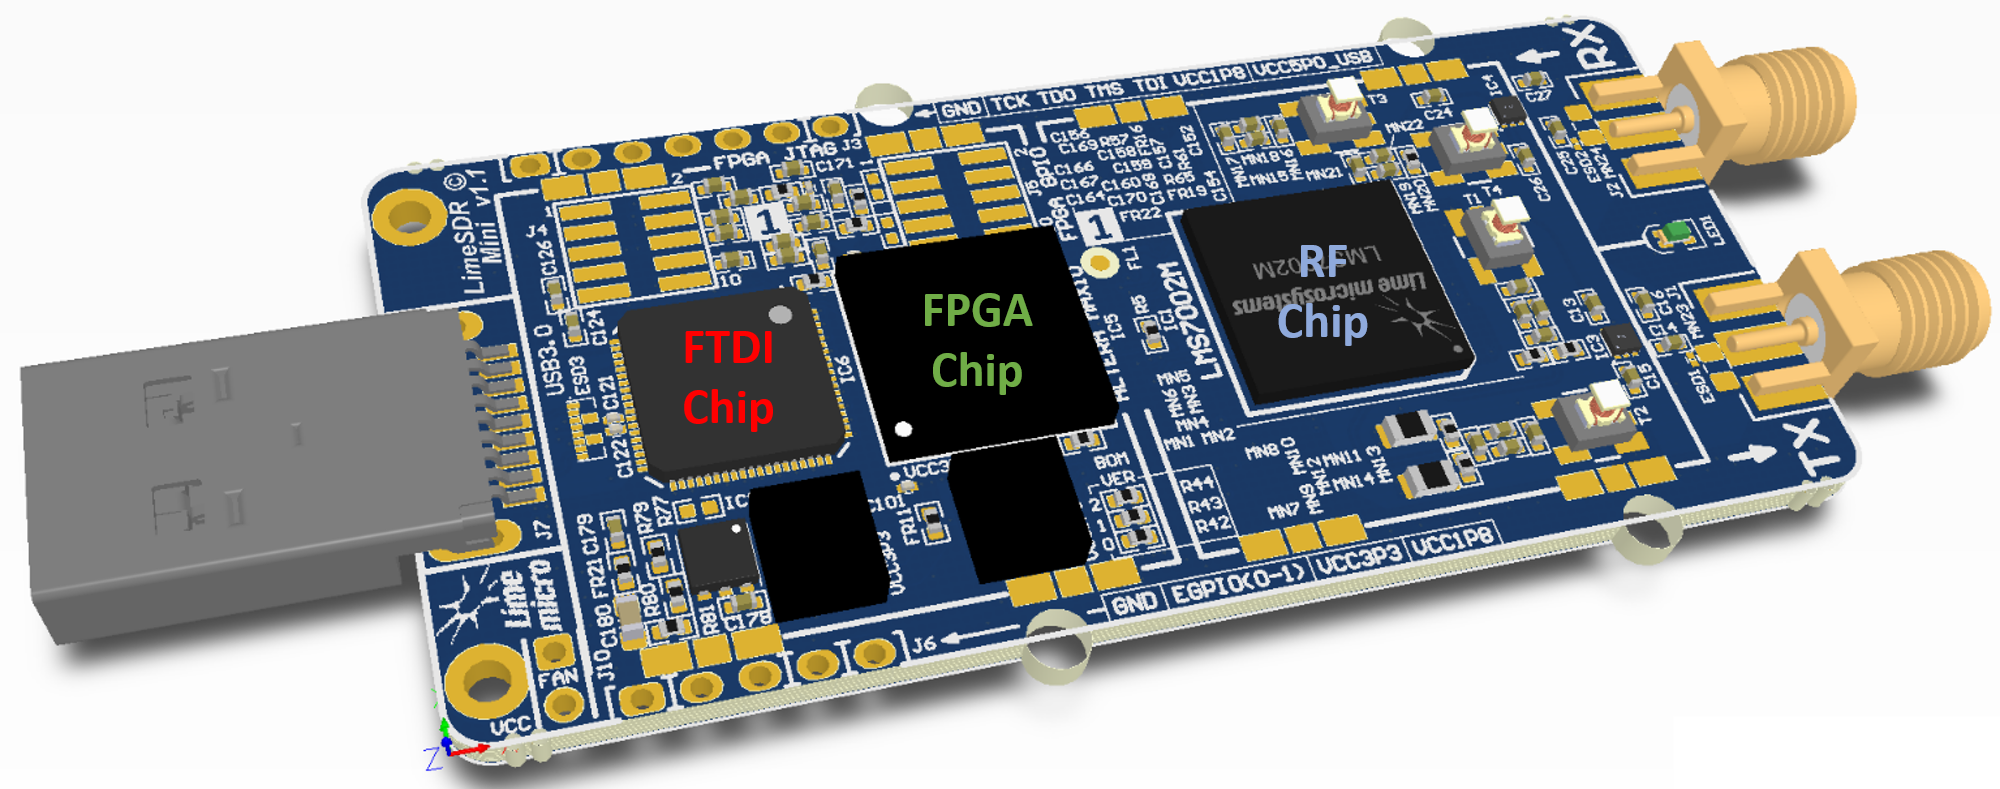
\includegraphics[width=0.7\linewidth]{figures/limesdrmini_schematic.png}
    \caption{Location of the different chips on the LimeSDR-Mini board.}
    \label{fig:limesdr_mini_schematic}
\end{figure}

\begin{figure}[!h]
    \centering
    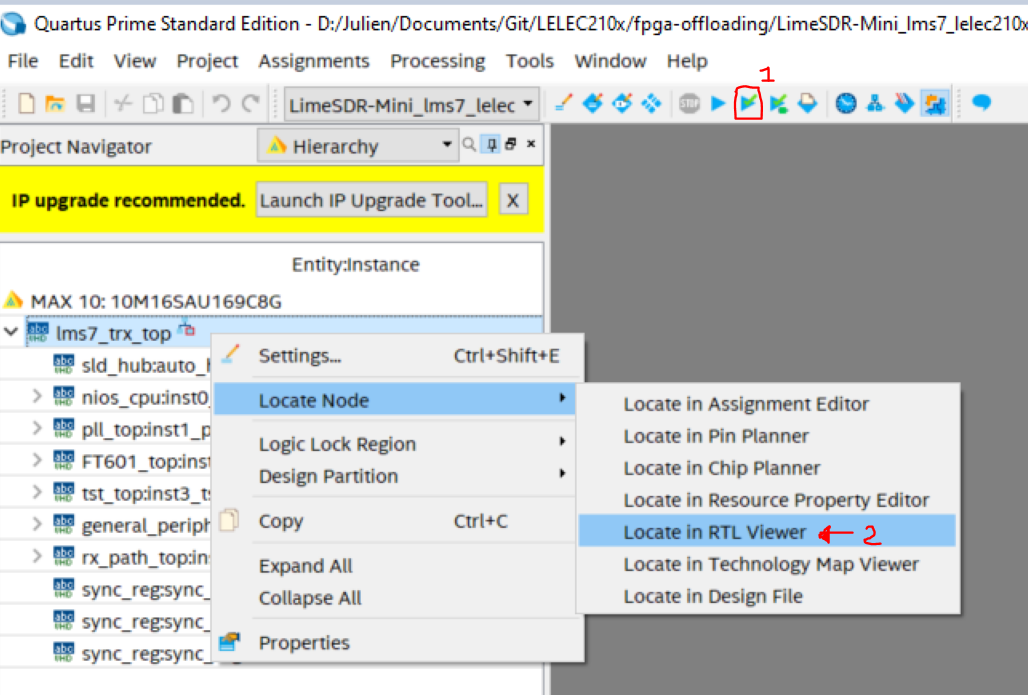
\includegraphics[width=0.7\linewidth]{figures/rtl_viewer.png}
    \caption{In order to use the RTL viewer, first elaborate the design (1) then right click on the design element you want view (2).}
    \label{fig:rtl_viewer}
\end{figure}

\section{Report R6}

The report R6 (due on \textbf{Nov 22, Monday 6.30 PM}). We expect you to:
\begin{itemize}
    \item Analyze with a graph, the number of cycles taken by the MAC function
        per authenticated byte for different message lengths : 1 byte up to 200
        bytes with steps of 1 byte. Do this for the different compiler
        optimization levels:
        \texttt{-O0},
        \texttt{-O1},
        \texttt{-O2},
        \texttt{-O3},
        \texttt{-Os}.\footnote{%
            To understand what these optimization levels do (as well as
            \texttt{-Og}), see
            \url{https://gcc.gnu.org/onlinedocs/gcc/Optimize-Options.html}.
            The optimizations controlled by these flags happen at the compiler
            level, and each file is compiled individually.

            Since optimization is based on gathering information on the
            code and how it is used, this limited (file-level) view may lead to
            missed optimization opportunities.
            Link-time optimization (LTO) is a technique that enables
            project-level view for optimizations (see
            \url{https://gcc.gnu.org/onlinedocs/gcc/Optimize-Options.html})
            and that you might want to use at some stage of your project.
            To add such custom compiler and linker flags, use the
            \textbf{Miscellaneous} section of the Compiler/Linker settings.
        }
    \item For the same optimization levels, analyze the code size of the
        authentication part of the project by comparing the total code size with
        and without authentication.
    \item Briefly discuss your results.
\end{itemize}



\end{document}
%%%%%%%%%%%%%%%%%%%%%%%%%%%%%%%%%%%%%%%%%%%%%%%%%%%%%%%%%%%%%%%%%%%%%%%%%%%%
